\documentclass[reprint, english,notitlepage,nofootinbib]{revtex4-1}  % defines the basic parameters of the document
% if you want a single-column, remove reprint

% allows special characters (including æøå)
\usepackage[utf8]{inputenc}
%\usepackage [norsk]{babel} %if you write norwegian
\usepackage[english]{babel}  %if you write english


%% note that you may need to download some of these packages manually, it depends on your setup.
%% I recommend downloading TeXMaker, because it includes a large library of the most common packages.

\usepackage{physics,amssymb}  % mathematical symbols (physics imports amsmath)
\usepackage{graphicx}         % include graphics such as plots
\usepackage{xcolor}           % set colors
\usepackage{hyperref}         % automagic cross-referencing (this is GODLIKE)
\usepackage{tikz}             % draw figures manually
\usepackage{listings}         % display code
\usepackage{subfigure}        % imports a lot of cool and useful figure commands
\usepackage{verbatim}
\usepackage{adjustbox}


% defines the color of hyperref objects
% Blending two colors:  blue!80!black  =  80% blue and 20% black
\hypersetup{ % this is just my personal choice, feel free to change things
    colorlinks,
    linkcolor={red!50!black},
    citecolor={blue!50!black},
    urlcolor={blue!80!black}}

%% Defines the style of the programming listing
%% This is actually my personal template, go ahead and change stuff if you want
\lstset{ %
	inputpath=,
	backgroundcolor=\color{white!88!black},
	basicstyle={\ttfamily\scriptsize},
	commentstyle=\color{magenta},
	language=Python,
	morekeywords={True,False},
	tabsize=4,
	stringstyle=\color{green!55!black},
	frame=single,
	keywordstyle=\color{blue},
	showstringspaces=false,
	columns=fullflexible,
	keepspaces=true}

\newcommand\numberthis{\addtocounter{equation}{1}\tag{\theequation}}
\newcommand{\ihat}{\boldsymbol{\hat{\textbf{\i}}}}
\newcommand{\jhat}{\boldsymbol{\hat{\textbf{\j}}}}
\newcommand{\khat}{\boldsymbol{\hat{\textbf{k}}}}
\newcommand{\del}[1]{\textbf{#1)}}
\newcommand{\svar}[1]{\underline{\underline{{#1}}}}
\newcommand{\vc}[1]{\mathbf{#1}}


\begin{document}


\begin{titlepage}
	\begin{center}
	\textbf{FYS3150 - Project 3}

	\vspace{0.2cm}
	Vegard Falmår and Sigurd Sørlie Rustad
	
	\vspace{0.5cm}
	
\includegraphics[scale=0.5]{UIO}
	\vspace{0.8cm}

	University of Oslo\\
	Norway\\
	\today	\\
	\end{center}
	\tableofcontents
	\clearpage
\end{titlepage}

\begin{abstract}
Abstract om du vil
\end{abstract}
\maketitle                              % creates the title


\section{Introduction}

In this report We will try to tackle many problems connected to planetary orbits. Everything from testing algorithms, to implementing general relativity. Planetary orbits and simulations are very relevant. An example of this is when we send probes far into space. Then we need to predict precise planetary orbits in order to do gravity assist maneuvers. Also being able to predict the initial velocity needed in order to escape the solar system is important. Therefore, in this report we are going to study different algorithms, looking at the conservation of energy and angular momentum. Using Velocity Verlet we will try to simulate many-many body problems, test for different gravitational forces, try to find the velocity needed to escape the gravitational field of our Sun and last but not least, study the perihelion precession of Mercury. We also have a theory section where you will find central concepts used in our report. A tentative list of our topics are also listed in the table of contents.
\\
Before we simulate systems, it is necessary to test our algorithm. Therefore, we test predictable scenarios, where we have more intuition on what the results should be. The tests we are going to do, are a binary system, namely the earth orbiting our Sun. We test for both circular and elliptical orbits, looking for conservation of energy and angular momentum. Running the simulation using Velocity Verlet and forward Euler, we can also compare algorithms.
\\
Studying many-body problems, we are mainly going to use data from NASA (see \citep{NASA}). We are mainly going to study two scenarios. First Earth, Sun and Jupiter, looking  at how different masses of Jupiter affects orbits. Then we look at all the planets in our solar system, including Pluto and Jupiter's moon Europa. For all scenarios we track the angular momentum and energy.
\\
We also found it interesting to explore how things would change with different gravitational forces. We know Newtons force of gravitation is proportional to one over $r$ squared ($F\propto1/r^2$). Where $r$ is the distance between two objects. We want to know how things would change if the force was proportional to ex. $1/r^3$. Thus we also look at different gravitational forces proportional to $1/r^n$, where $n\in\{2,3\}$.
\\
Like we mentioned above, knowing the velocity needed to escape a gravitational potential is important. We are going to study a situation where we have a theoretical value. Namely an object, one astronomical unit away from our Sun. The theoretical calculations are covered in our theory section. In our studies we are going to test for initial velocities, and try to find the lowest velocity that escapes the gravitational potential of our Sun. Then compare it to the theoretical value we calculated.
\\
As we will cover in the theory section, Newton's force of gravitation cannot explain the observed precession of Mercury's orbit. Implementing a general relativistic correction into our force, we can simulate Mercury's orbit for 100 years, and study the precession. Our hope is to predict this observed precession in our simulations.
\\
For our studies we have used c++ for heavy computation, python for visualization and bash for automation. All the code along with instructions on how to run it, can be cloned from our GitHub repository here\footnote{github.com/sigurdru/FYS3150/tree/master/Project2}.

\section{Theory}

\subsection{Newton's laws and the motion of planets}

The well-known Newtons second law reads
\begin{equation}
  \label{eq:Newton_2nd}
  \sum \vc F = m \frac{\mathrm d^2 \vc r}{\mathrm d t^2},
\end{equation}
where $\sum \vc F$ is the sum of forces acting on an object, $m$ is its mass and $\vc r$ its position.
\\
Newton's law of gravity says that the total gravitational force acting on an object $i$ from all the other objects in a system is
\begin{equation}
  \label{eq:Newton_grav}
  F_{G, i} = - G m_i \sum_{j \neq i} m_j \frac{\vc r_i - \vc r_j}{ \lvert \vc r_i - \vc r_j \rvert ^3}
\end{equation}
where $\vc r_i$ are the positions and $m_i$ are the masses of the objects. $G$ is the gravitational constant.
\\
For the motions of planets, on which the gravitational force is the only force acting, the two equations \ref{eq:Newton_2nd} and \ref{eq:Newton_grav} combined give us the differential equation that describes the motion of an object:
\begin{equation}
  \label{eq:DE}
  \frac{\mathrm d^2 \vc r_i}{\mathrm d t^2} = \frac{1}{m_i} F_{G, i} = - G \sum_{j \neq i} m_j \frac{\vc r_i - \vc r_j}{ \lvert \vc r_i - \vc r_j \rvert ^3}
\end{equation}


\subsection{Velocity Verlet}

Classical problem of Newtonian mechanics often involve solvinga set of two coupled first order differential equations, namely
\begin{align*}
  \frac{\mathrm d x}{\mathrm dt} = v \\
  \frac{\mathrm d v}{\mathrm dt} = a
\end{align*}
where $x$ is position, $v$ is velocity and $a$ is acceleration. Doing a Taylor expansion of $x$ around a point in time $t = t_0$ gives
\begin{align*}
  x(t) &= x(t_0) + (t - t_0) \frac{\mathrm d x}{\mathrm dt}(t_0) + \frac{1}{2} (t - t_0)^2 \frac{\mathrm d^2 x}{\mathrm dt^2}(t_0) + O(h^3) \\
  &= x(t_0) + (t - t_0) v(t_0) + \frac{1}{2} (t - t_0)^2 a + O(h^3)
\end{align*}
An expression can then be found for position at a time $t = t_0 \pm h$:
\begin{equation}
  \label{eq:Taylor_exp_x}
  x(t_0 \pm h) = x(t_0) \pm h v(t_0) + \frac{1}{2} h^2 a \pm O(h^3)
\end{equation}
\\
Discretizing equation \ref{eq:Taylor_exp_x} and letting $x_i = x(t)$, $x_{i+1} = x(t + h)$, $v_i = v(t)$ and $v_{i+1} = v(t + h)$, we get
\begin{align*}
  x_{i+1} \approx x_i + h v_i + \frac{h^2}{2} a_i \\
  v_{i+1} \approx v_i + h a_i + \frac{h^2}{2} \dot a_i,
\end{align*}
where $\dot a_i$ is the derivative of the acceleration with respect to time. Similarly to the case of Forward Euler, doing a Taylor expansion of $a$ gives after some manipulation
\begin{equation}
  \dot a_i \approx \frac{a_{i+1} - a_i}{h}
\end{equation}
Insering this into the expressions we have for $x_{i+1}$ and $v_{i+1}$ gives us the equations that describe the Velocity Verlet method:
\begin{align*}
  x_{i+1} \approx x_i + h v_i + \frac{h^2}{2} a_i \\
  v_{i+1} \approx v_i + \frac{h}{2} (a_{i+1} + a_i)
\end{align*}
From equation \ref{eq:Taylor_exp_x} we see that the mathematical error in this approximation goes like $O(h^3)$.


\subsection{Forward Euler}

From equation \ref{eq:Taylor_exp_x} we see that by including only the two first terms in the Taylor expansion of $x(t)$ and $v(t)$ we get
\begin{align*}
  x_{i+1} \approx x_i + h v_i \\
  v_{i+1} \approx v_i + h a_i
\end{align*}
This is referred to as the Forward Euler method of solving differential equations. The mathematical error in this approximation goes like $O(h^2)$.


\subsection{Conservation of angular momentum and energy}

Kepler's second law states that if you draw a line from the Sun to a planet orbiting it, then that line would sweep out the same area in equal periods of time. We will use this law to derive the conservation of angular momentum.
\\
For short periods of time $\mathrm d t$ the area swept out by the line from the Sun to the planet is approximately a triangle with area
\begin{equation*}
  A = \frac{1}{2} r v_\theta \mathrm dt
\end{equation*}
where $r$ is the distance from the planet to the Sun and $v_\theta$ is the tangential velocity of the planet. Kepler's second law states that this area is constant for all intervalls of time of the same length. For this to be true, we must require
\begin{equation*}
  r v_\theta = \text{constant}
\end{equation*}
The angular momentum $\vc L$ of the planet around the Sun is
\begin{align*}
  \vc L &= \vc r \times \vc p \\
  &= r \ihat_r \times m(v_\theta \ihat_\theta + v_r \ihat_r) \\
  &= m r v_\theta \khat, \quad \text{as } \ihat_r \times \ihat_\theta = \khat \text{ and } \ihat_r \times \ihat_r = 0 \\
  &= \text{constant}
\end{align*}
\\
Newton's gravitational force is conservative, therefore the energy of our system should be conserved. Kinetic energy is given by
\begin{equation}
\label{eq:kinetic_energy}
K = \frac{1}{2}mv^2,
\end{equation}
where $K$ is the kinetic energy, $m$ is the mass and $v$ is the velocity. The potential energy of an object (with reference point set to infinity) in a gravitational field is given by
\begin{equation}
\label{eq:potential_energy}
U = G\sum_{i}\frac{Mm_i}{r_i}
\end{equation}
Where $U$ is the potential energy, $G$ the gravitational constant, $r_i$ the relative distance between the objects, $m_i$ mass of an object creating the gravitational field, and $M$ mass of the object we want to find the energy of.

\subsection{Escape velocity}

The inverse square law of gravity (Newton's law of gravity) is a conservative force with a potential
\begin{equation}
  \label{eq:pot_G}
  U_G(r) = - G \frac{m_1 m_2}{r}
\end{equation}
The sum of this potential energy and the kinetic energy will be conserved for celestial objects. In order to escape the gravitational pull of the Sun, a planet in orbit must have a total energy $E = U_G + K \ge 0$ as the potential energy goes to zero infinitely far away:
\begin{align*}
  E = U_G + K &\ge 0 \\
  K &\ge - U_G \\
  \frac{1}{2} M v^2 &\ge G \frac{M M_\odot}{r} \\
  v &\ge \sqrt{G \frac{2 M_\odot}{r}}
\end{align*}
A planet which begins at a distance 1 AU from the Sun, will therefore need an initial velocity of
\begin{align*}
  v_0 &= \sqrt{G \frac{2 M_\odot}{1 \text{ AU}}} \\
  &= \sqrt{8 \pi^2 \frac{\text{AU}^2}{\text{yr}^2}} \\
  &= 2 \sqrt 2 \pi \frac{\text{AU}}{\text{yr}} \numberthis \label{eq:escape_velocity}
\end{align*}
in order to be able to escape the gravitational pull of the Sun.

\subsection{Adjusting speed and position of the center of mass}
When you have a planetary system, all the planets orbit a common center of mass. This point can have a velocity, meaning that if we don't account for it, the system will drift when we simulate. There are many ways to account for this drift, however we choose to adjust the velocity of all the objects, such that there are none. In order to do this you first have to find the velocity. This is done by first finding the momentum
\begin{equation*}
	\mathbf{p}_{\text{CM}} = \sum_{i=1}^{n}m_i\mathbf{v_i}
\end{equation*} 
and then dividing by the total mass of the system
\begin{equation}
	\label{eq:v_cm}
	\mathbf{v}_{\text{CM}} = \frac{1}{M}\mathbf{p}_{\text{CM}} =  \frac{1}{M}\sum_{i=1}^{n}m_i\mathbf{v_i}.
\end{equation} 
Where $\mathbf{p}_{\text{CM}}$ and $\mathbf{v}_{\text{CM}}$ is the momentum and velocity of the center of mass. $M$ the total mass of the system, $n$ the number of planets and, $m_i$ and $\mathbf{v_i}$ the mass and velocity of the individual planets. By subtracting $\mathbf{v}_{\text{CM}}$ from the velocity of every planet, the center of mass should not drift. Similarly, we can place the origin in the center of mass. This is done by first finding the position:
\begin{equation}
	\label{eq:r_cm}
	\mathbf{r}_{\text{CM}} =  \frac{1}{M}\sum_{i=1}^{n}m_i\mathbf{r_i},
\end{equation}
where $\mathbf{r}_{\text{CM}}$ is the center of mass position and $r_i$ the individual planets positions. Then we can do the same as above, subtract $\mathbf{r}_{\text{CM}}$ from the positions of all the planets. Then with the center of mass placed in the origin with zero velocity, it should not move.

\subsection{The perihelion precession of Mercury}
We know, because of general relativity, that Newtons law of gravitation is not entirely correct. An example of where we see this effect is in the precession of Mercury's perihelion. Even when taking into account the gravitational force from all the other planets in the solar-system, Newtons law of gravitation cannot explain how the perihelion moves around the Sun. Therefore, when we have relativistic effects, we add a correction. For binary systems this becomes (see \citep{oppgavetekst})
\begin{equation}
	\label{eq:general_relativity}
	F_{1 \rightarrow 2} = \frac{GM_1M_2}{r^2}\left[ 1 + \frac{3l^2}{r^2c^2} \right].
\end{equation}
Where $F_{1 \rightarrow 2}$ is the force acting from object one on two, $G$ the gravitational constant, $M_1$ and $M_2$ are the masses of object one and two, $r$ their relative position, $l$ the magnitude of object two's orbital angular momentum and $c$ the speed of light.

\section{Methods}

\subsection{Discretization of the equations of motion}

Equation \ref{eq:DE} is the equation of motion that describes the system of planets and stars in motion. We want to solve this equation numerically for all the planets in our solar system. In order to do this we must discretize the equations. We can rewrite the equation as a set of first order differential equations using the velocity:
\begin{align*}
   \frac{\mathrm d \vc r}{\mathrm d t} &= \vc v \\
   \frac{\mathrm d \vc v}{\mathrm d t} &= - G \sum_{j \neq i} m_j \frac{\vc r_i - \vc r_j}{ \lvert \vc r_i - \vc r_j \rvert ^3}
\end{align*}
\\
The Verlet is not a self-starting algorithm.
Mainly applicable when we are not interested in the velocity
Velocity Verlet is energy conserving, Forward Euler is not


\subsection{Units of measurement}

Measuring distance in meters and time in seconds leads to very large numbers when doing calculations on the solar system. In order to do our calculations with numbers of magnitudes closer to $10^0$, we will measure time in years and distance in astronomical units AU, which is the mean distance between the Sun and the Earth. For an object in circular motion with radius $R$ and period $T$, the acceleration is given by the sentripetal acceleration
\begin{equation*}
  a = \frac{v^2}{r} = \frac{(2 \pi R / T)^2}{R} = \frac{4 \pi^2 R}{T^2}
\end{equation*}
With a small error, we can model the orbit of the Earth around the Sun as circular. To further simplify the expressions, we will measure masses in solar masses $M_\odot$. For the Earth's orbit we have $R = 1$ AU and $T = 1$ yr. This means that the force acting on the Earth from the Sun is
\begin{align*}
  F_{G, \text{Earth}} &= G \frac{M_{\text{Earth}} M_\odot}{\text{AU}^2} \\
  &= M_{\text{Earth}} a_{\text{Earth}} \\
  &\approx M_{\text{Earth}} \frac{4 \pi^2 \text{AU}}{\text{yr}^2} \\
  G &\approx 4 \pi^2 \frac{\text{AU}^3}{M_\odot \text{yr}^2}
\end{align*}
In units of AU, $M_\odot$ and yr the gravitational constant has a value of approximately $4 \pi$.

\subsection{The data from NASA}
When we study orbits in our solar-system, we want them to be realistic. Therefore we use actual data from NASA (see \citep{NASA}), that provides us the real positions, velocities and masses of planets and moons in our solar system. The data shows positions and velocities from the perspective of the barycenter, which is the center of mass. In our solvers, we still adjust for , because it allows us to test for data which does not have this property. 

\subsection{Testing and comparing algorithms}
In order to make sure our algorithms runs correctly, we want to test it. During testing, we also use the opportunity to look at differences between forward Euler and Velocity Verlet. Therefore we do the tests with both algorithms. Our first test will be to simulate the simplest possible system, namely earth orbiting the Sun. We place the Sun in origin and with zero velocity. The earth orbits with a distance of $r=1$AU away from the Sun, and makes a full orbit every year. This gives it an initial velocity of $v = 2\pi \text{ AU}/\text{yr}.$ This system however will have a center of mass that drifts. In order to counteract this we will move the origin to where the center of mass is, and zero its velocity. See the theory section on how this is done.
\\
Testing for different time steps $\Delta t$, we can look at the stability of velocity Verlet and Euler's forward method. Now we have to decide on what constitutes a stable orbit. Even though we adjust the barycenters drift, this effect is neglishable and we should still expect the earths orbit to have a distance of 1AU away from the barycenter. Therefore we will test for different $\Delta t$ and see how the distance varies from our expected value. We do each test over 10 years, and calculate the difference every $0.01/\Delta t$ steps (100 times).
\\
Another test will be conservation of kinetic and potential energy. As mentioned above, the earth should have a constant distance away from the barycenter, meaning potential energy is conserved. Earths speed should also be the same, meaning kinetic energy stays the same. Therefore, we will test for this as well. 
\\
The last test of our algorithm will be conservation of angular momentum. In the theory section, from Kepler's second law, we showed that angular momentum is conserved. Therefore we will also test whether that is the case for our Earth-Sun system. Adding some complexity, as well as testing it for the near ideal orbit over, we tested conservation of angular momentum with the initial conditions collected from NASA (see \citep{NASA}).

\subsection{Different forms of gravitational force}

\subsection{Escape velocity}
An interesting test to do, is to see if we can find the escape velocity. We found the analytical term in the theory section (see equation \eqref{eq:escape_velocity}), for an object 1AU away from our Sun. We can test for different initial velocities, se for what velocity the planet escapes, then compare to the analytical result. There are two things we have to decide, how we test for different velocities, and how do we know whether or not we have the right velocity.
\\
From the analytical term we know that a speed of 8AU/yr should be bound. Therefore that will be the first velocity, and increase with 0.01AU/yr, until we have escaped. The initial velocity will always point radially away from the Sun, to make the simulation easier. Because the initial velocity is pointing radially away from the Sun, we know it is not bound, if the velocity ever points back towards the Sun in our simulation.
\\
Now how do we know if a planet has escaped? We know that to be the case analytically, when the potential energy is zero. However we cannot be that precise in our simulations. Therefore we decide on a tolerance, such that if the planet has a lower potential energy than the tolerance, we say the planet has escaped.

\subsection{Many-body problem}

\subsection{General relativity}
Like we discussed in the theory section, newtons law of gravitation is not entirely correct. For example it does not explain the precession of Mercury's orbit. Therefore we try to implement an relativistic correction into our model (see equation \eqref{eq:general_relativity}). From \citep{oppgavetekst} we know that the observed value for Mercury's perihelion precession is around $43''$. This is with all interactions from other planets accounted for. Therefore, we are going to see if we can reproduce this, with only Mercury and the Sun. We neglect the gravitational interactions on the Sun, because it is around seven orders of magnitude larger than Mercury. With this in mind we can place the stationary Sun in origin, and from \citep{oppgavetekst} we have the initial conditions for Mercury. Starting velocity is 12.44AU/yr in the y-direction, and an initial position in its perihelion, an x-position of 0.3075AU.
\\
We do the simulation for 100 years, and then find the new perihelion. We cannot guarantee that Mercury is in the perihelion after 100 years, therefore we let the simulation go on for around 90 more days (reassuring us that Mercury completes another orbit), then finding the closest position to the Sun (which is the perihelion). With the new position of the perihelion, we can easily calculate its precession with
\begin{equation*}
	\tan(\theta_P) = \frac{y_P}{x_P}.
\end{equation*}
Where $\theta_P$ is precession angle, $x_P$ and $y_P$ is the x- and y-position of the new perihelion.
\\
Because we are running the simulation for such a long time, we use Velocity Verlet. Choosing a low enough time step is the biggest challenge. Our solution to this is testing for different time steps and comparing the results. Lowering it by a factor of 10$^{-1}$ until we are satisfied, or until the computation time takes over an hour.

\section{results}

\subsection{Testing and comparing algorithms}



\subsection{Different forms of gravitational force}

\begin{figure}[h]
	\centering
	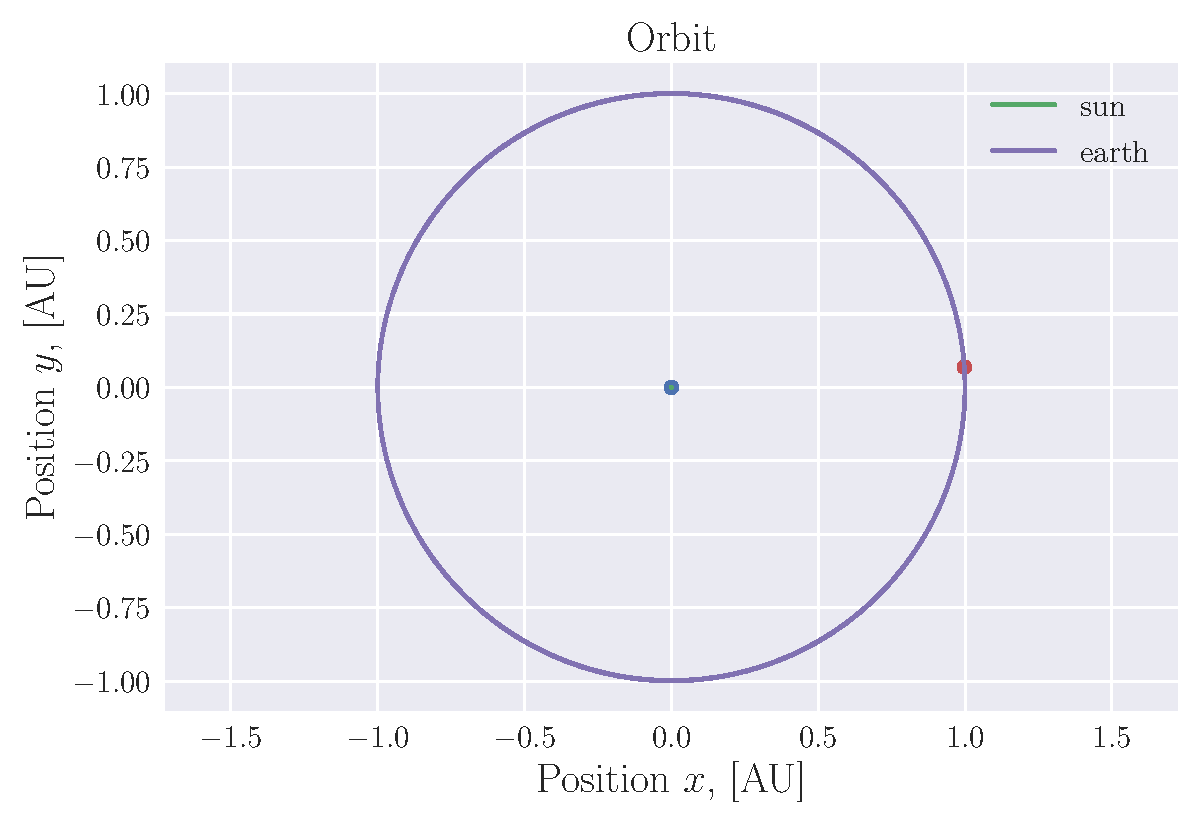
\includegraphics[width=\linewidth]{../output/earth_sun_circ-verlet-3-5-2_75.pdf}
	\caption{In this figure 
		\label{fig:betha=2_75}}
\end{figure}

\begin{figure}[h]
	\centering
	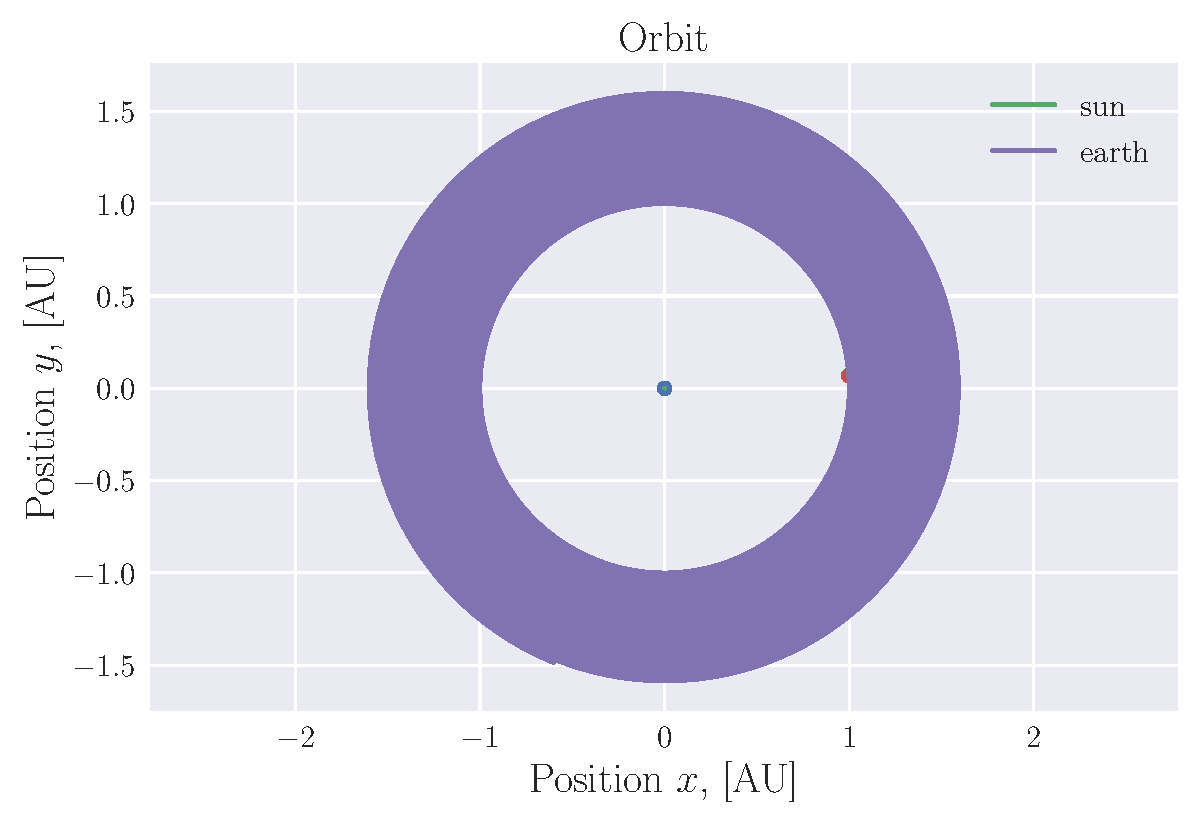
\includegraphics[width=\linewidth]{../output/earth_sun_circ-verlet-3-5-3.pdf}
	\caption{In this figure 
		\label{fig:betha=3}}
\end{figure}

\begin{figure}[h]
	\centering
	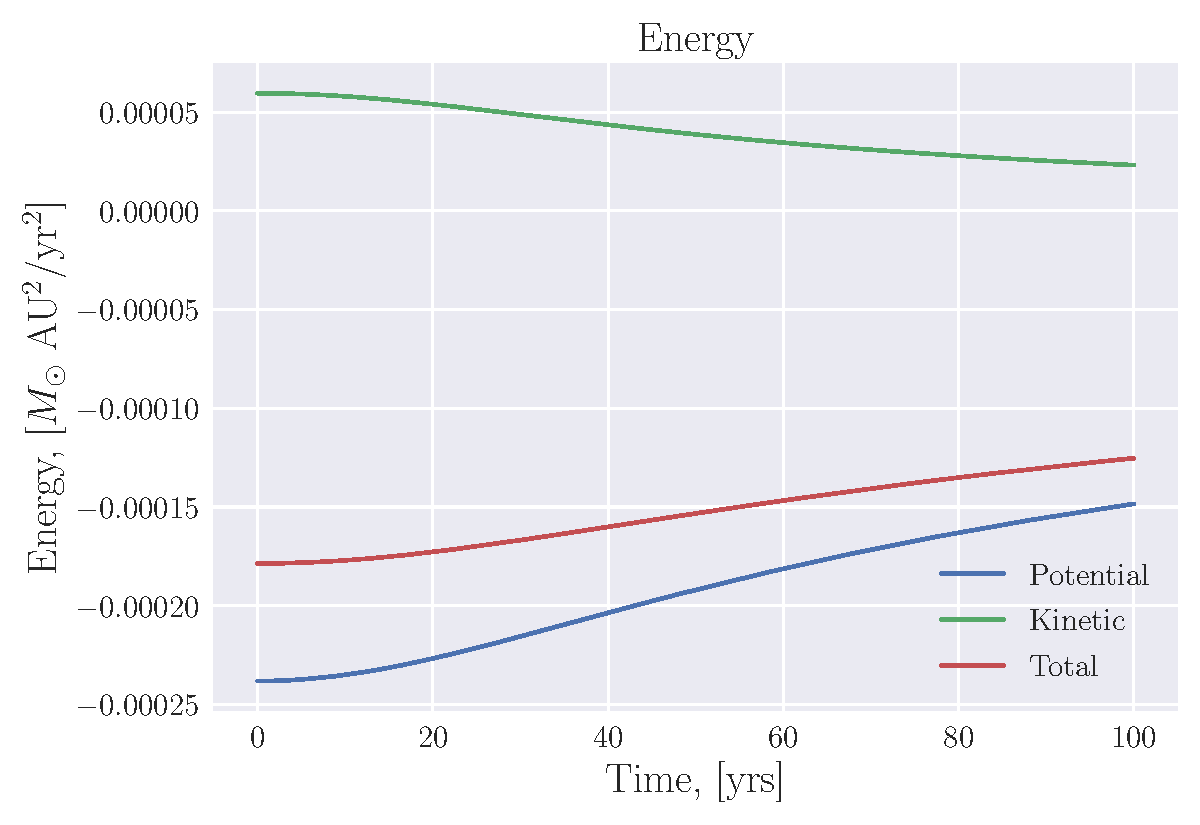
\includegraphics[width=\linewidth]{../output/earth_sun_circ-verlet-3-5-3_energy.pdf}
	\caption{In this figure 
		\label{fig:betha=3_energy}}
\end{figure}

\begin{figure}[h]
	\centering
	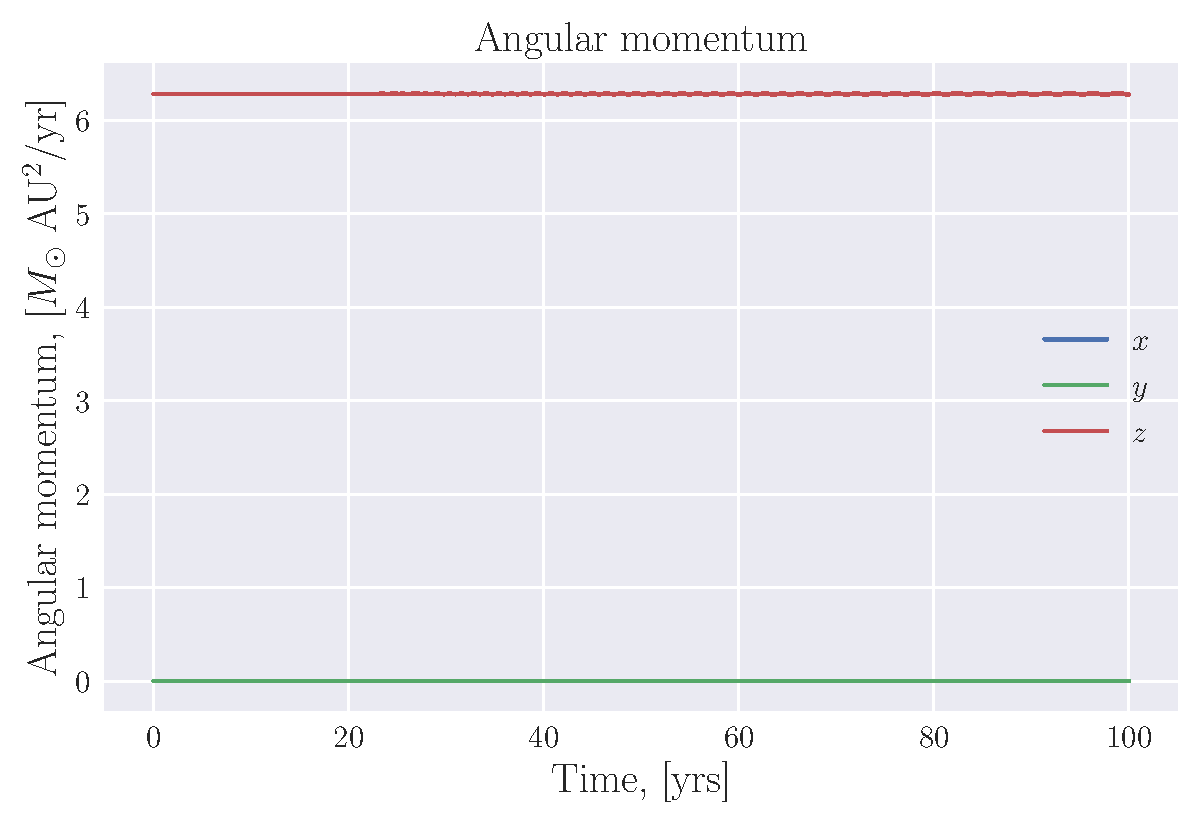
\includegraphics[width=\linewidth]{../output/earth_sun_circ-verlet-3-5-3_ang_mom.pdf}
	\caption{In this figure 
		\label{fig:4}}
\end{figure}

\subsection{Escape velocity}
The theoretical escape velocity is known to be $V_{\text{teo}} = 2\pi\sqrt{2} \approx 8.89$AU/yr (this is from equation \eqref{eq:escape_velocity}). When finding the escape velocity we had to test for different tolerances. Lower gave more precise results, however at the cost of computation time. We found that with a tolerance of $\epsilon = 0.001$M$_\odot$AU$^2$/yr$^2$ we got a escape velocity of $v_{\text{esc}} = 8.89$AU/yr, which corresponds to the theoretical value. Time step during simulation was set to $10^{-4}$yr.


\subsection{Many-body problem}

\begin{figure}[h]
	\centering
	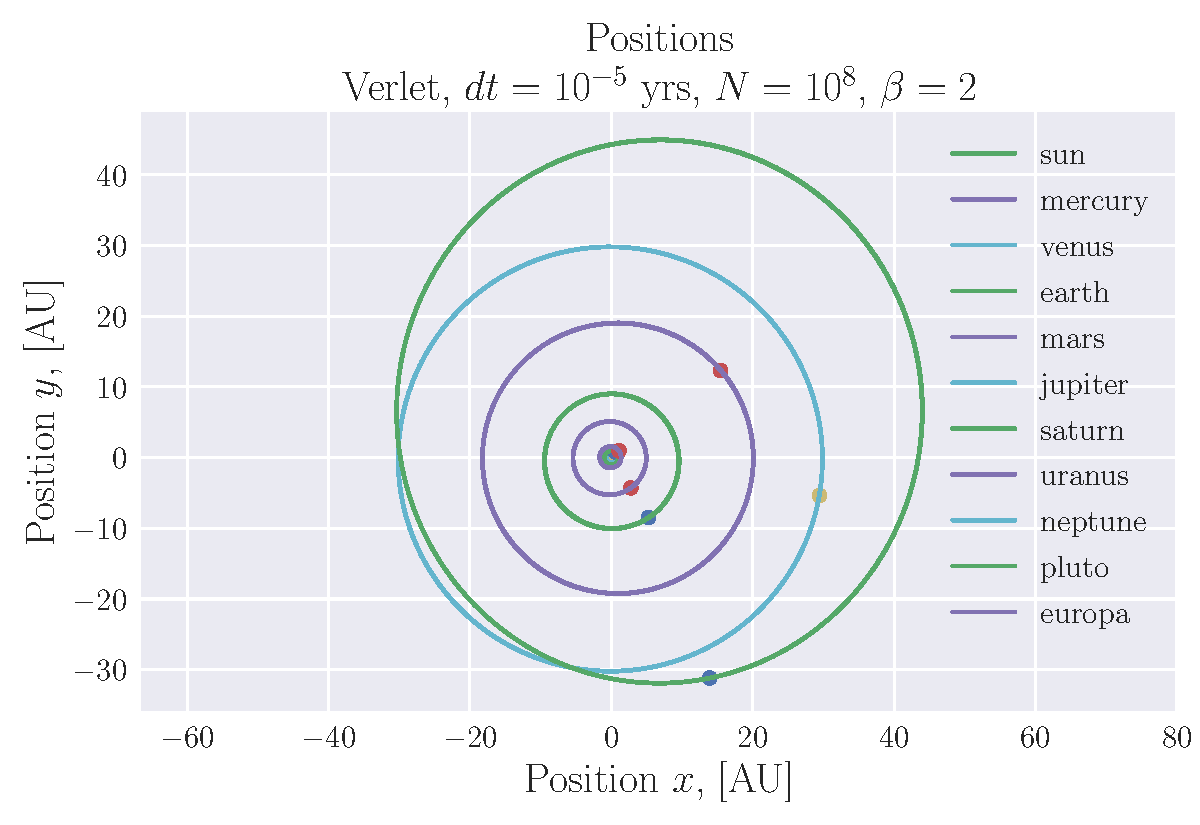
\includegraphics[width=\linewidth]{../output/all-verlet-5-8-2.pdf}
	\caption{In this figure 
		\label{fig:all}}
\end{figure}

\begin{figure}[h]
	\centering
	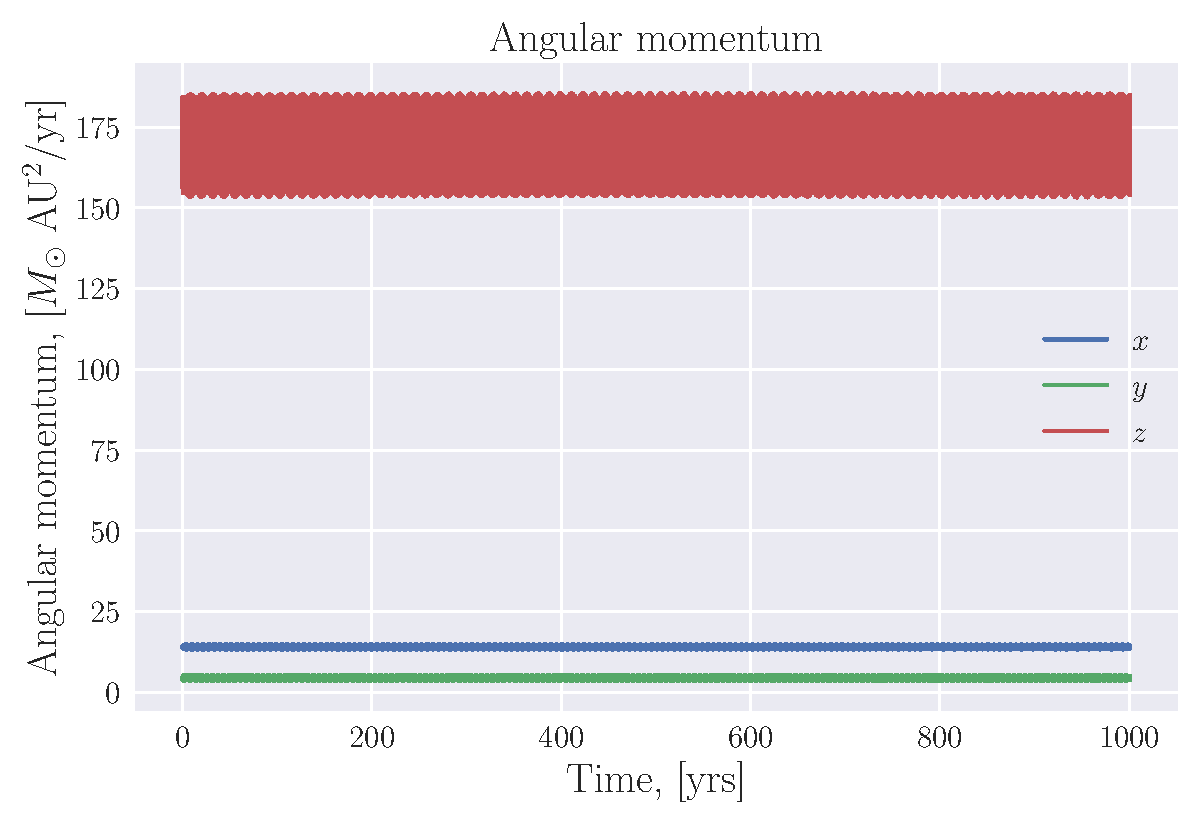
\includegraphics[width=\linewidth]{../output/all-verlet-5-8-2_ang_mom.pdf}
	\caption{In this figure 
		\label{fig:all_ang_mom}}
\end{figure}

\begin{figure}[h]
	\centering
	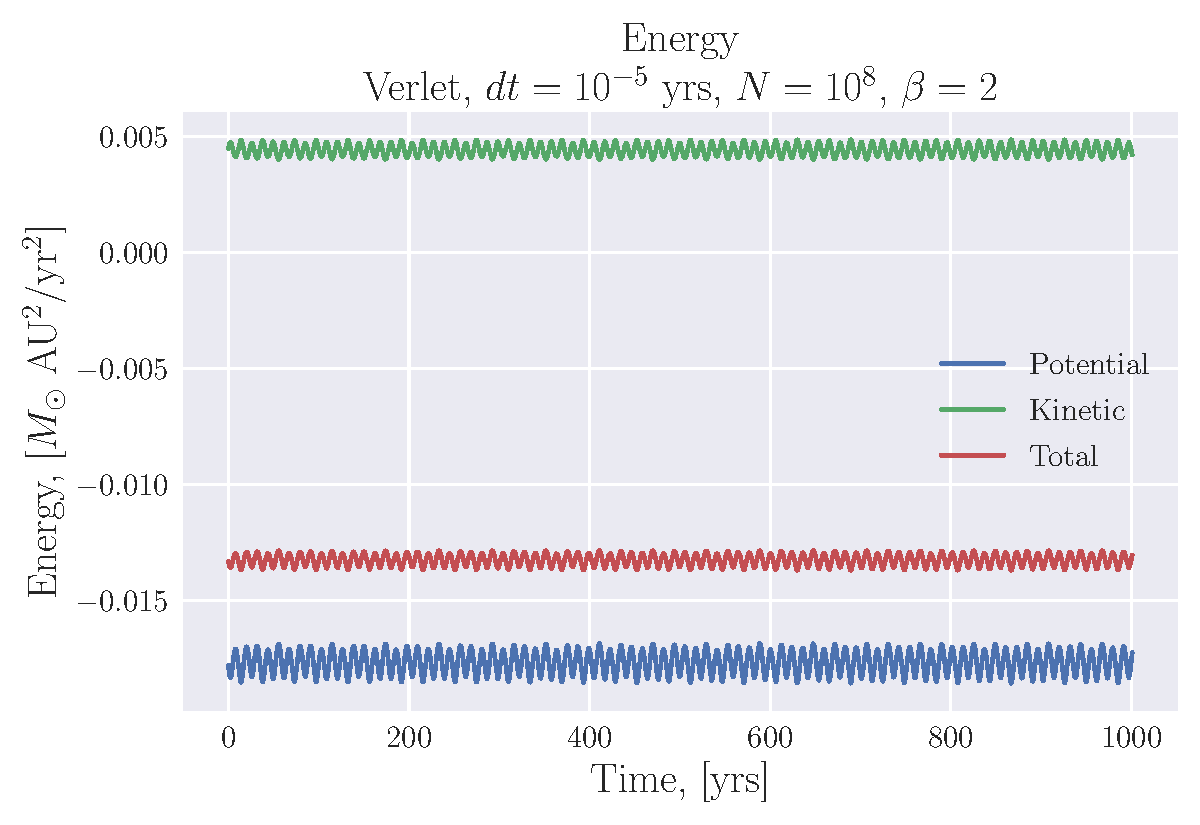
\includegraphics[width=\linewidth]{../output/all-verlet-5-8-2_energy.pdf}
	\caption{In this figure 
		\label{fig:all_energy}}
\end{figure}

\subsection{General relativity}

We ended up doing the tests for three different time steps (see \ref{tab:general_relativity}). Notice that with a time step of around 3.16 seconds, we got a precession of 43.26$''$ which is quite close to the theoretical value of 43$''$. Time step of 31.56 seconds was also quite close, with a value of 40.43$''$. Our first result however, showed precession in the opposite direction.
\begin{table}[h]
	\begin{tabular}{|l|l|l|}
		\hline
		Timestep {[}s{]} & Integration points N & Result {[}arcseconds{]} \\
		\hline
		315.56              & $10^7$          & -0.79               \\
		31.56               & $10^8$          & 40.43                 \\
		3.16                & $10^9$          & 43.26	\\
		\hline                
	\end{tabular}
	\caption{In this table you have the different time steps we tested for, in units of seconds. The second column shows the number of integration points needed, and the last column is our results in arcseconds. 
	\label{tab:general_relativity}}
\end{table}
\\
We wanted to test for smaller time steps, however we exceeded the maximum array-length. Also, because our last result were quite close to the theoretical, we opted against it.

\section{discussion}

testing and comparing algorithms(discuss eventual differences between the verlet algorithm and the euler algorithm. Consider also the numver of flops involved and perform a timing of the two algorithm for equal final times.)

different forms of gravitation

As we mentioned, when calculating the escape velocity, we cannot be infinitely precise. There is a constant trade-off between precision and computation time. We don't believe our method and calculations are wrong, as we are studying a very simple system. What we do acknowledge however, is that we could get a more precise answer.

many body problem

When including a general relativistic correction, we ended up at the observed value. However it is worth discussing the fact that we only arrived at the right answer for one time step, namely 3.16 seconds. Ideally we would want to test for lower time steps, to confirm that this was not a fluke. However, seeing that we arrived very close for the time step 31.56 seconds, it seems unlikely.

\section{conclusion}




\onecolumngrid
\vspace{1cm} % some extra space
\newpage

\begin{thebibliography}{}
\bibitem[]{oppgavetekst} Department of Physics, Univeristy of Oslo, Fall semester 2020, Computational Physics I FYS3150/FYS4150, Project 3.
\bibitem[]{NASA} Ryan S. Park, Alan B. Chamberlin, NASA, 27. October 2020, https://ssd.jpl.nasa.gov/horizons.cgi\#top.

\end{thebibliography}


\end{document}
